\documentclass[compress]{beamer}
\usepackage[english,russian]{babel}
\usepackage[utf8]{inputenc}
\usepackage{pagenumber}

\usepackage{hyperref}
% Стиль презентации
\usetheme[numbers, totalnumbers]{Dresden}
% цветовая схема
\usecolortheme{beaver}

\newcommand\Fontvi{\fontsize{6}{7.2}\selectfont}

\makeatletter
\defbeamertemplate*{footline}{Dresden}{
	\leavevmode%
	\hbox{%
	\begin{beamercolorbox}[wd=0.88\paperwidth,ht=2.25ex,dp=1ex,center]{title in head/foot}%
		\usebeamerfont{title in head/foot}\inserttitle
	\end{beamercolorbox}%
	\begin{beamercolorbox}[wd=.12\paperwidth,ht=2.25ex,dp=1ex,right]{date in head/foot}%
		\usebeamerfont{date in head/foot}\hspace*{2em}
		\insertframenumber{} / \inserttotalframenumber\hspace*{2ex}
	\end{beamercolorbox}}%
}
\defbeamertemplate*{headline}{Dresden}{
}
\makeatother

\begin{document}
\title{Пространственно-кинематическое моделирование однородной плоской подсистемы Галактики}  
\author{Д.В. Волков}
\institute{Научный руководитель: к.\,ф.-м.\,н., доцент кафедры небесной механики \\ И.И. Никифоров}
\date{Санкт-Петербургский государственный университет, \\Кафедра небесной механики \\ \today} 
% Создание заглавной страницы
\frame{\titlepage} 

\begin{frame}{Модельные предположения}
	\begin{enumerate}
                \item Средняя линейная скорость $\Theta$ вращения подсистем Галактики -- функция галактоосевого расстояния $R$: $\Theta = \Theta (R)$ (цилиндрический закон вращения).
                \item Невязки (отклонения) наблюдаемых скоростей от их модельных значений распределены по нормальному закону с нулевым математическим ожиданием. 
                \item Порядок разложения $n$ аппроксимирующих закон вращения полиномов не фиксируется заранее, а оптимизируется в ходе решения.
                \item Ни для каких параметров модели не принималось никаких внешних предположений. Вектор параметров модели $\textbf{p} = (R_0,~u_{\odot},~v_{\odot},~w_{\odot},~\omega_0,~A, \ldots, \theta_n)$.
	\end{enumerate}
\end{frame}

\begin{frame}{Полиномиальная модель вращения}
Для представления $\Theta(R)$ используем модельный полином в виде многочлена Тейлора:
	\begin{equation}
		\Theta_n(R) = \sum^n_{k = 0} \frac{\theta_k}{k!} \left( \Delta R \right)^k,
	\end{equation}
где
\begin{equation}
        \Delta R = R - R_0, \qquad \theta_k = \frac{d^k\Theta}{dR^k},
\end{equation}
\begin{equation}
	R = \sqrt{R_0^2 + r^2 \cos^2{b} - 2R_0 r \cos{l} \cos{b}}.
\end{equation}
Здесь и далее $l$ -- галактическая долгота, $b$ -- галактическая широта, $r$ -- гелиоцентрическое расстояние.
\end{frame}

\begin{frame}{Модель для поля лучевых скоростей}
\begin{equation}
        V_{r, \mathrm{mod}} = (\omega - \omega_0) R_0 \sin{l} \cos{b} - V_{r, \odot},
\end{equation}
где $\omega$ и $\omega_0$ -- угловые скорости вращения подсистемы на $R$ и $R_0$,  $V_{r, \odot}$ -- проекция остаточной скорости движения Солнца на луч зрения:
\begin{equation}
        V_{r, \odot} = -u_{\odot} \cos{l} \cos{b} - v_{\odot} \cos{b} \sin{l} - w_{\odot} \sin{b}.
\end{equation}
$u_{\odot}, v_{\odot}, w_{\odot}$ -- проекции остаточного движения Солнца на направления $(l, b) = (0^{\circ}, 0^{\circ})$, $(l, b) = (90^{\circ}, 0^{\circ})$ и $b = 90^{\circ}$ соот\-ветст\-вен\-но.
	\begin{equation}
		V_{r, \mathrm{mod}} = \left[ -2A\Delta R + \sum^n_{k = 2} \frac{\theta_k}{k!} \left( \Delta R \right)^k \right] \frac{R_0}{R} \sin{l} \cos{b} + V_{r, \odot},
	\end{equation}
	\begin{equation}
		A = - \frac{1}{2} R_0 \omega^{'}(R_0) = - \frac{1}{2} (\theta_1 - \omega_0).
	\end{equation}
\end{frame}

\begin{frame}{Модель для собственных движений по галактической долготе}
Для собственных движений $\mu_l = \frac{dl}{dt}\cos{b}$:
\begin{equation}
        k\mu_{l, \mathrm{mod}} = (\omega - \omega_0) \left( \frac{R_0\cos{l}}{r} - \cos{b} \right) - \omega_0 \cos{b} + k\mu_{l, \odot},
\end{equation}
	\begin{equation}
		k\mu_{l, \mathrm{mod}} = k\mu_{l, \mathrm{rot}} + k\mu_{l, \odot},
	\end{equation}
	\begin{multline}
                k\mu_{l, \mathrm{rot}} = \left[ -2A\Delta R + \sum^n_{k = 2} \frac{\theta_k}{k!} \left( \Delta R \right)^k \right] \left( \frac{R_0\cos{l}}{r} - \cos{b} \right) R^{-1} -\\
                -\omega_0 \cos{b},
	\end{multline}
	\begin{equation}
                k\mu_{b, \odot} = \frac{u_{\odot}\sin{l}- v_{\odot}\cos{l}}{r}.
	\end{equation}

        Здесь и далее полагаем $k=4.7406$ км/с.
\end{frame}


\begin{frame}{Модель для собственных движений по галактической широте}
Для собственных движений $\mu_b = \frac{db}{dt}$:
\begin{equation}
        \mu_{b, \mathrm{mod}} = - (\omega - \omega_0) \frac{R_0}{r} \sin{l} \sin{b} + \mu_{b, \odot}.
\end{equation}
	\begin{equation}
		k\mu_{b, \mathrm{mod}} = k\mu_{b, \mathrm{rot}} + k\mu_{b, \odot},
	\end{equation}
	\begin{equation}
		k\mu_{b, \mathrm{rot}} = \left[ 2A\Delta R - \sum^n_{k = 2} \frac{\theta_k}{k!} \left( \Delta R \right)^k \right] \frac{R_0}{Rr} \sin{l} \sin{b},
	\end{equation}
	\begin{equation}
                k\mu_{b, \odot} = \frac{u_{\odot}\cos{l}\sin{b} + v_{\odot}\sin{l}\sin{b} - w_{\odot}\cos{b}}{r}.
	\end{equation}
\end{frame}

\begin{frame}{Раздельные решения}
	Решаются системы уравнений
	\begin{equation}
                V_r = V_{r, \mathrm{mod}} (R_0, A, \theta_2, \:\ldots,\: \theta_n, u_{\odot}, v_{\odot}, w_{\odot}^{*}),
	\end{equation}
	\begin{equation}
                k\mu_l = k\mu_{l, \mathrm{mod}} (R_0^{*}, A, \omega_0, \theta_2, \:\ldots,\: \theta_n, u_{\odot}, v_{\odot}),
	\end{equation}
	\begin{equation}
                k\mu_b = k\mu_{b, \mathrm{mod}} (R_0^{*}, A, \theta_2, \:\ldots,\: \theta_n, u_{\odot}, v_{\odot}, w_{\odot}).
	\end{equation}
        Параметры со звездочкой могут фиксироваться. Каждая из систем решается обычным МНК с единичными весами.
\end{frame}

\begin{frame}{Раздельные решения}
        Минимизируются следующие статистики:
	\begin{equation}
                \sigma^2_{V_r} = \frac{1}{N_{\mathrm{free}}} \sum^N_{i = 1} \left( V_r - V_{r, \mathrm{mod}} \right)^2_i,
	\end{equation}
	\begin{equation}
                \sigma^2_{\mu_l} = \frac{1}{N_{\mathrm{free}}} \sum^N_{i = 1} \left( k\mu_l - k\mu_{l, \mathrm{mod}} \right)^2_i,
	\end{equation}
	\begin{equation}
                \sigma^2_{\mu_b} = \frac{1}{N_{\mathrm{free}}} \sum^N_{i = 1} \left( k\mu_b - k\mu_{b, \mathrm{mod}} \right)^2_i,
	\end{equation}
        где число степеней свободы $N_{\mathrm{free}} = N - n_{\mathrm{par}}$, $n_{\mathrm{par}}$ -- количество параметров модели.
\end{frame}

\begin{frame}{Совместное решение по трем компонентам скоростей}
\textit{Природная дисперсия} $\sigma_0$ объектов подсистемы -- дисперсия скоростей, обусловленная динамикой звездной системы, а не ошибками измерений. Минимизируется целевая функция
\begin{multline} \label{chi_sq_func}
        \chi^2 (\sigma_0) = \\ 
                          \quad=\sum^N_{i = 1} \left[ \frac{\left( V_r - V_{r, \mathrm{mod}} \right)^2_i}{\sigma_0^2 + \sigma^2_{V_{r_i}}} + \frac{\left(k \mu_l - k\mu_{l, \mathrm{mod}} \right)^2_i}{\frac{\sigma_0^2}{r_i^2} + k^2\sigma^2_{\mu_{l_i}}} + \frac{\left(k \mu_b - k\mu_{b, \mathrm{mod}} \right)^2_i}{\frac{\sigma_0^2}{r_i^2} + k^2\sigma^2_{\mu_{b_i}}} \right].
\end{multline}

\par Здесь $\sigma_{V_{r_i}}$, $\sigma_{\mu_{l_i}}$, $\sigma_{\mu_{b_i}}$ -- ошибки измерения лучевых скоростей и собственных движений.

\begin{equation}
        \chi^2(\sigma_0) |_{\sigma_{0, \mathrm{opt}}} = N_{\mathrm{free}} = 3 N - n_{\mathrm{par}}.
\end{equation}
\end{frame}


\begin{frame}{Выбор оптимального порядка полинoма}
	Критерии.
	\begin{itemize}
		\item Значимость старших коэффициентов.
		\item Зависимость дисперсии от порядка.
		\item Наличие краевых эффектов у кривой вращения для данного порядка.
                \item Гладкость профиля 
                        \begin{equation}
                        \chi^2_m(R_0) = \min_{R_0 = \mathrm{const}} \chi^2(\textbf{p}) 
                        \end{equation}
                        целевой функции для параметра $R_0$ .
                \item Связность линий равной плотности маргинальных распределений параметров.
	\end{itemize}
\end{frame}

\begin{frame}{Исключение по невязкам}
	\begin{itemize}
		\item Для данного объема выборки вычисляется значение $\kappa$
			\begin{equation}
				\big(1 - \psi(\kappa)\big) N = 1,
			\end{equation}
			где $\psi(\kappa)$ -- интеграл вероятностей:
			\begin{equation}
				\psi(\kappa) = \sqrt{\frac{2}{\pi}} \int^{\kappa}_{0} e^{-\frac{1}{2}t^2} dt.
			\end{equation}
		\item Исключаются объекты с невязками
			\begin{equation}
				\frac{| \varepsilon_i |}{\sigma_i} > \kappa
			\end{equation}
	\end{itemize}
        Далее находится количество объектов $L$, удовлетворяющих условию. Если $L > 1$, то из дальнейшего рассмотрения исключается $L - 1$ объектов с наибольшими по модулю невязками (Никифоров, 2012). 
\end{frame}

\begin{frame}{Единицы измерения}
        Для дальнейшего удобства договоримся о том, что значения следующих величин и их неопределенностей, если не указано иначе, приводятся в следующих единицах.
        \begin{itemize}
                \item Любые расстояния ($r$, $R$, $R_0$ и т.д.) в кпк.
                \item Линейные скорости ($\Theta$, $V_r$, $u_{\odot}$, $v_{\odot}$, $w_{\odot}$) в км/с.
                \item Угловые скорости ($\omega_0$, $\omega_{\odot}$) в км/c/кпк.
                \item Собственные движения $\mu_l, ~\mu_b$ в мсд/год.
                \item Величина $A$ в км/c/кпк.
        \end{itemize}
\end{frame}

\begin{frame}{Наблюдательные данные}
        Красное сгущение -- высокометалличный аналог горизонтальной ветви, образуемой населением II типа. Paczynski, Stanek (1998) предложили использовать звезды красного сгущения как новый индикатор расстояний.
	\begin{center}
	\begin{figure}[h]
\begin{minipage}[h]{0.65\linewidth}
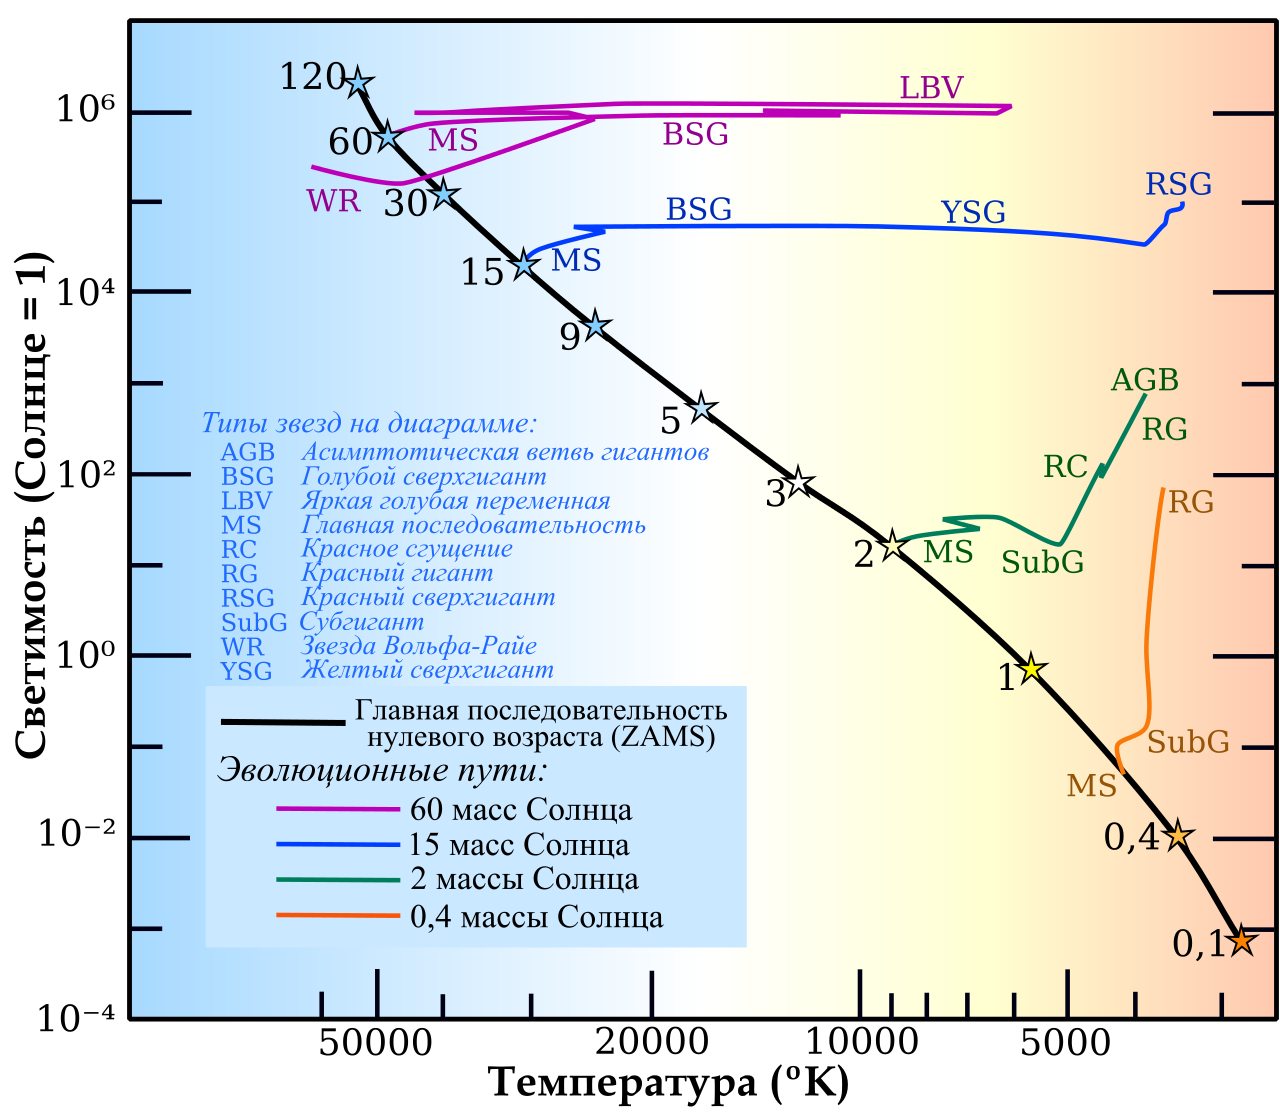
\includegraphics[width=1\linewidth]{../imgs/Stellar_evolutionary_tracks-rus.png}
\end{minipage}
\end{figure}
	\end{center}
\end{frame}


\begin{frame}{APOGEE-RC}
        Apache Point Observatory Galactic Evolution Experiment (APOGEE) представляет собой спектроскопию в ближней инфракрасной области с высоким разрешением, охватывающую все основные компоненты Галактики, в том числе экранируемые пылью области внутреннего диска и балджа Галактики. Каталог RC (Red Clump)  -- результат работы Bovy+(2014). Данные APOGEE-RC для ЗКС: фотометрические расстояния с точностью от $5$ до $10\%$ в калибровке $M_{K_s} = -1.613 \pm 0.015 $ (Laney, 2012), что на 0.07 зв. вел. ярче, чем у Groenewegen (2008); гелиоцентрические расстояния, лучевые скорости, и собственные движения из каталогов UCAC-4 и HSOY (Hot Stuff for One Year). 
\end{frame}



\begin{frame}{APOGEE-RC}

Распределение объектов APOGEE-RC в гeлиоцентрических декартовых координатах. Ось $X$ ориентирована на центр Галактики.
\begin{figure}[h!]
\begin{minipage}[h]{0.49\linewidth}
        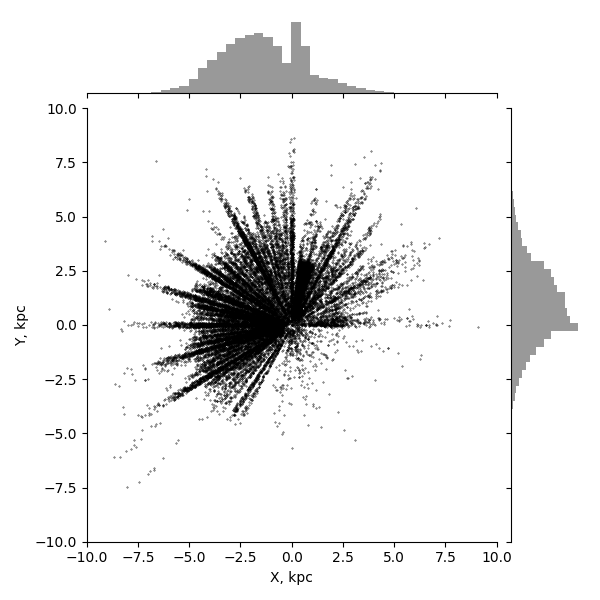
\includegraphics[width=0.95\textwidth]{../imgs/XYobj.png}
\end{minipage}
\hfill
\begin{minipage}[h]{0.49\linewidth}
        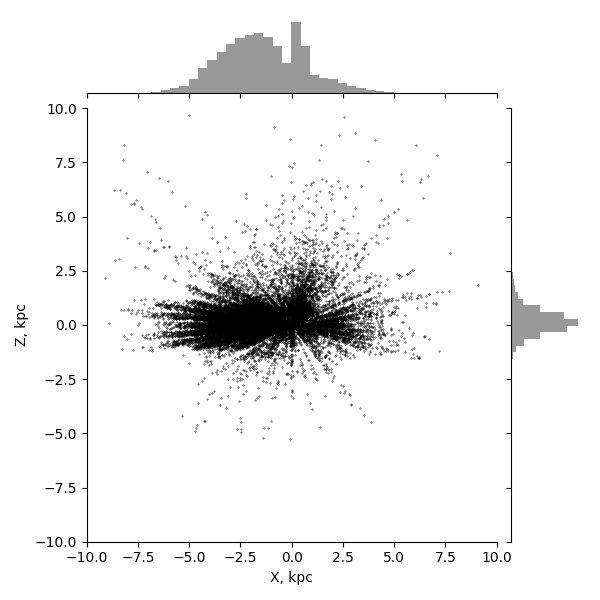
\includegraphics[width=0.95\textwidth]{../imgs/XZobj.png}
\end{minipage}
\end{figure}


\end{frame}


\begin{frame}{Результаты раздельного решения по лучевым скоростям}
\Fontvi
\begin{table}[h!!]
\centering
\begin{tabular}{r|rr|r|rrrrrr}
\hline
 $n$ & $1$ & $2$ & $3$ & $4$ & $5$&$ 6 $&$ 7 $&$ 8 $&$ 9 $\\\hline
 $R_0 $& 8.167       &   7.515 &   7.611 &   7.487 &   7.616 &   7.797 &   7.806 &   7.822 &   7.528  \\
       & $_{-0.113}^{+0.132} $ & $_{-0.052}^{+0.051}$  & $_{-0.143}^{+0.245}$   & $_{-0.075}^{+0.092}$  & $_{-0.144}^{+0.258}$  & $_{-0.064}^{+0.096}$  & $_{-0.065}^{+0.097}$  & $_{-0.070}^{+0.105}$  & $_{-0.043}^{+0.042}$  \\\hline
 $\sigma_{V_r} $& 32.189      &  32.213 &  32.117 &  32.103 &  32.096 &  32.108 &  32.117 &  32.118 &  32.112  \\
 $ u_{\odot} $& 12.412      &  12.275 &  12.688 &  12.754 &  12.785 &   12.81 &  12.807 &  12.805 &  12.814  \\
 $\sigma_{u_{\odot}} $&0.270       &   0.265 &   0.267 &   0.267 &   0.261 &   0.269 &    0.270 &   0.267 &   0.253  \\
 $v_{\odot} $& 29.601      &  28.161 &   26.98 &  27.271 &  27.098 &  27.643 &  27.769 &  27.763 &  26.871  \\
 $\sigma_{v_{\odot}}$&0.358       &   0.393 &    0.470 &   0.458 &   0.491 &   0.527 &   0.505 &   0.518 &   0.462  \\
 $w_{\odot} $&6.698       &   6.894 &    7.320 &   7.372 &   7.524 &   7.522 &   7.446 &   7.434 &   7.614  \\
 $\sigma_{w_{\odot}} $& 0.636       &   0.615 &   0.633 &   0.639 &   0.619 &    0.610 &    0.630 &   0.663 &    0.660  \\\hline
 $A $&13.013      &  12.969 &  14.491 &  15.022 &  15.279 &  15.662 &  15.612 &  15.459 &  15.345  \\
 $\sigma(A) $ & 0.128     &    0.130 &   0.174 &   0.206 &   0.209 &   0.262 &   0.262 &   0.306 &   0.318  \\
 $\theta_2$&-        &  -0.974 &  -2.038 &  -1.156 &  -1.776 &  -0.842 &  -0.549 &  -0.624 &  -2.635  \\
 $\sigma(\theta_2)$&-      &   0.169 &   0.222 &   0.279 &   0.343 &   0.423 &   0.558 &   0.536 &   0.731  \\
 $\theta_3$&-      &    - &   2.009 &   2.655 &   3.385 &   4.322 &   4.101 &   3.523 &   2.825  \\
 $\sigma(\theta_3)$&-      &    - &   0.147 &   0.192 &   0.270 &   0.403 &   0.480 &   0.814 &   0.843  \\
 $\theta_4$&-      &    - &    - &  -0.681 &  -0.184 &  -1.227 &  -1.561 &  -1.297 &   2.809  \\
 $\sigma(\theta_4)$&-      &    - &    - &   0.132 &   0.183 &   0.346 &   0.560 &   0.601 &   1.265  \\
 $\theta_5$&-      &    - &    - &    - &  -0.498 &  -0.946 &  -0.645 &   0.073 &   0.392  \\
 $\sigma(\theta_5)$&-      &    - &    - &    - &   0.132 &   0.189 &   0.423 &   0.936 &   1.017  \\

 \end{tabular}
\end{table}

\end{frame}


\begin{frame}{Результаты раздельного решения по долготным собственным движениям}
\Fontvi
По пересечению с каталогом HSOY
\begin{table}[h!!]
\centering
\begin{tabular}{r|rrr|r|rrrrr}
\hline
$n$ & $1$ & $2$ & $3$ & $\textbf{4}$ & $5$&$ 6 $&$ 7 $&$ 8 $&$ 9 $\\\hline
 $N_{\mathrm{end}}$ & 28378       &   28377 &   28378 &   28378 &   28379 &   28379 &   28378 &   28378 &   28377 \\
 $R_0 $& 6.718*      &   8.185 &   8.792 &   8.694 &   8.732 &   8.726 &    8.590 &   8.744 &   8.733 \\
       & $_{-0.067}^{+0.067} $ & $_{-0.387}^{+0.462}$ & $_{-0.444}^{+0.286}$   & $_{-0.398}^{+0.337}$  & $_{-0.409}^{+0.303}$  & $_{-0.401}^{+0.312}$  & $_{-0.438}^{+0.404}$  & $_{-0.437}^{+0.307}$  & $_{-0.358}^{+0.339}$  \\\hline
 $\sigma_{\mu_l} $& 22.956      &  22.884 &  22.879 &  22.874 &  22.881 &  22.881 &  22.875 &  22.875 &  22.868  \\ 
 $ u_{\odot} $& 11.563      &  11.808 &  11.679 &  11.658 &  11.636 &   11.65 &  11.644 &  11.622 &  11.564  \\
 $\sigma_{u_{\odot}} $&0.484       &   0.492 &    0.49 &   0.493 &   0.484 &   0.487 &   0.487 &   0.497 &   0.498  \\
 $v_{\odot} $& 20.519      &  21.075 &  19.982 &  19.934 &   19.75 &  19.816 &  19.957 &   19.79 &  19.805  \\
 $\sigma_{v_{\odot}}$&0.462       &   0.429 &   0.494 &   0.498 &   0.522 &   0.576 &   0.572 &   0.601 &   0.608  \\
 $\omega_0 $&29.275      &  28.786 &  28.842 &  28.908 &  28.911 &  28.908 &  28.902 &  28.905 &  28.889  \\
 $\sigma_{\omega_0} $& 0.346       &   0.376 &   0.369 &   0.373 &   0.364 &   0.363 &   0.366 &   0.371 &   0.368  \\\hline
 $A $&15.953      &  13.636 &  13.988 &  14.447 &  14.456 &  14.395 &  14.495 &  14.604 &  14.705  \\
 $\sigma(A) $ & 0.234       &   0.295 &   0.307 &   0.333 &   0.325 &   0.364 &   0.378 &    0.420 &   0.442  \\
 $\theta_2$&-        &  -3.161 &  -4.465 &  -3.917 &  -4.185 &  -4.152 &  -3.642 &  -3.959 &  -3.627  \\
 $\sigma(\theta_2)$&-      &    0.209 &   0.321 &   0.359 &   0.463 &   0.489 &   0.685 &   0.693 &   0.748  \\
 $\theta_3$&-      &    - &   1.075 &   1.643 &   1.785 &   1.598 &   1.729 &   2.329 &   2.652  \\
 $\sigma(\theta_3)$&-      &    - &   0.203 &   0.252 &   0.298 &   0.585 &   0.668 &   0.925 &   1.117  \\
 $\theta_4$&-      &    - &    - &  -0.527 &  -0.398 &  -0.337 &  -1.051 &  -0.870 &  -1.692  \\
 $\sigma(\theta_4)$&-      &    - &    - &    0.148 &   0.235 &   0.266 &   0.743 &   0.774 &   1.196  \\
 $\theta_5$&-      &    - &    - &    - &  -0.096 &  -0.005 &   0.163 &  -0.639 &  -0.744  \\
 $\sigma(\theta_5)$&-      &    - &    - &    - &    0.126 &   0.292 &   0.337 &   0.990 &   1.157  \\

 \end{tabular}
\end{table}
\end{frame}


\begin{frame}{Сопоставление результатов раздельных решений}
        $K_A \equiv \frac{A_{V_r}}{A_{\mu_l}}$ для допустимых порядков.
\begin{table}[h!!] 
\centering
\begin{tabular}{r|rrr}
        $ n$ & 3 & 4 & 5 \\
\hline
\hline
$A_{V_r} $& $14.491     $&  $  15.022$ & $ 15.279 $ \\
$\sigma_{A_{V_r}}$& $0.174 $    &  $0.206 $& $  0.209  $\\
$A_{\mu_l} $& $13.988 $    & $ 14.447$ & $14.456 $ \\
$\sigma_{A_{\mu_l}}$& $0.307 $    & $0.333 $& $0.325 $ \\
\hline
$K_A$& $1.036 $    &   $1.040 $& $ 1.057 $ \\
$ \sigma_{K_A}$& $0.035 $    & $0.035 $&  $0.038 $ 
\end{tabular}
\end{table}

Взвешенное среднее ${<}K_A{>} = 1.044 \pm 0.036$.
\end{frame}




\begin{frame}{Результаты совместного решения по трехмерному полю скоростей}
\Fontvi
По пересечению с каталогом HSOY
\begin{table}[h!!] \label{table_hsoy_sigma0}
\begin{tabular}{r|rr|r|r|r|rrrrr}
\hline
$n$ & $1$ & $2$ & $3$ & $4$ & $5$&$ 6 $&$ 7 $&$ 8 $&$ 9 $\\\hline
 $R_0 $& \textbf{8.509}       &     \textbf{7.520} &   \textbf{7.548} &   \textbf{7.458} &   \textbf{7.483} &   \textbf{7.539} &     \textbf{7.540} &   \textbf{7.529} &   \textbf{7.831} \\
       & $_{-0.155}^{+0.194} $ & $_{-0.040}^{+0.038}$ & $_{-0.089}^{+0.066}$   & $_{-0.050}^{+0.055}$  & $_{-0.092}^{+0.113}$  & $_{-0.117}^{+0.082}$  & $_{-0.067}^{+0.053}$  & $_{-0.029}^{+0.031}$  & $_{-0.026}^{+0.029}$  \\\hline
 $\sigma_0 $& 20.984      &  21.013 &  20.983 &  20.963 &  20.959 &  20.961 &  20.955 &  20.959 &  20.972  \\ 
 $\sigma_{\Theta} $& 53.154      &  53.268 &  53.873 &  53.350 &  53.323 &  53.377 &  53.281 &  53.283 &  53.345  \\\hline 
 $ u_{\odot} $& 12.410      &   12.227 &  12.473 &  12.565 &  12.575 &  12.583 &   12.604 &  12.607 &  12.594 \\
 $\sigma_{u_{\odot}} $&0.181       &     0.180 &   0.181 &   0.174 &   0.177 &   0.181 &    0.181 &   0.175 &    0.170 \\
 $v_{\odot} $& 30.372      &   28.257 &  27.145 &  27.452 &  27.204 &  27.257 &   27.641 &  27.545 &    27.800 \\
 $\sigma_{v_{\odot}}$&0.232       &    0.256 &   0.297 &   0.283 &   0.306 &   0.305 &    0.295 &   0.315 &   0.308 \\
 $w_{\odot} $& 7.148       &    7.391 &   7.659 &   7.709 &   7.774 &   7.816 &    7.768 &   7.818 &   7.768 \\
 $\sigma_{w_{\odot}}$&0.346       &    0.339 &   0.338 &   0.354 &   0.345 &   0.331 &    0.367 &   0.349 &   0.351 \\
 $\omega_0 $&25.838      &   27.008 &  26.929 &  26.847 &  26.839 &   26.790 &   26.774 &  26.798 &  26.562 \\
 $\sigma_{\omega_0} $& 0.226       &     0.230 &   0.249 &   0.231 &   0.251 &   0.244 &    0.241 &   0.235 &   0.233 \\\hline
 $A $&12.825      &   12.646 &   13.630 &  14.328 &  14.419 &  14.652 &    14.82 &  14.995 &  14.504 \\
 $\sigma(A) $ & 0.087       &    0.087 &    0.110 &   0.129 &   0.132 &   0.152 &    0.156 &   0.179 &     0.200 \\
 $\theta_2$&-        &  -1.489 &  -2.419 &  -1.474 &  -1.975 &  -1.894 &   -0.806 &  -1.117 &  -1.568 \\
 $\sigma(\theta_2)$&-      &     0.102 &    0.130 &   0.158 &   0.198 &   0.219 &     0.310 &   0.347 &    0.410 \\
 $\theta_3$&-      &    - &   1.319 &   2.163 &   2.478 &   3.086 &    3.187 &   3.943 &   2.312 \\
 $\sigma(\theta_3)$&-      &    - &   0.081 &   0.124 &   0.144 &   0.225 &    0.235 &   0.390 &   0.455 \\
 $\theta_4$&-      &    - &    - &  -0.740 &  -0.413 &  -0.634 &   -1.899 &  -1.654 &   0.162 \\
 $\sigma(\theta_4)$&-      &    - &    - &     0.072 &   0.104 &   0.133 &    0.313 &   0.347 &   0.600 \\
 $\theta_5$&-      &    - &    - &    - &  -0.240 &  -0.578 &   -0.287 &  -1.288 &   0.460 \\
 $\sigma(\theta_5)$&-      &    - &    - &    - &     0.057 &   0.113 &    0.128 &   0.452 &   0.467 \\

 \end{tabular}
\end{table}
\end{frame}

\begin{frame}{Итоговые оценки основных характеристик кинематической модели}
\begin{table}[h!!] 
\centering
\begin{tabular}{r||r|r}
       &  $K_A = 1.000$ & $K_A = 1.044$\\
\hline
\hline
$A $&  $ 13.96 \pm 0.18 $& $13.08 \pm 0.10$ \\ 
$u_{\odot} $ & $12.52 \pm 0.17  $& $ 12.45 \pm 0.16$\\
$v_{\odot} $  & $27.17  \pm 0.30 $& $27.09 \pm 0.28$\\
$w_{\odot} $ & $7.71 \pm 0.34$ & $7.77 \pm 0.34$\\
\hline
$R_0  $ & \textbf{7.516} $^{+0.072}_{-0.090} $   & \textbf{7.838} $^{+0.101}_{-0.088}$ \\
$\omega_0 $ & $26.88 \pm 0.25 $ & $26.07 \pm 0.23$\\
$\theta_0 $& $202.2 \pm 4.2 $ & $ 204.3 \pm 4.3$ \\
\hline
$\omega_{\odot} $& $30.50 \pm 0.33 $ & $29.53 \pm 0.31$ \\
$\theta_{\odot} $& $229.2 \pm 4.9 $ & $231.4 \pm 5.2$ \\
\end{tabular}
\end{table}

\end{frame}


\begin{frame}{Кривая вращения}
\begin{figure}[h!!]
\begin{center}
\begin{minipage}[p]{0.65\linewidth}
        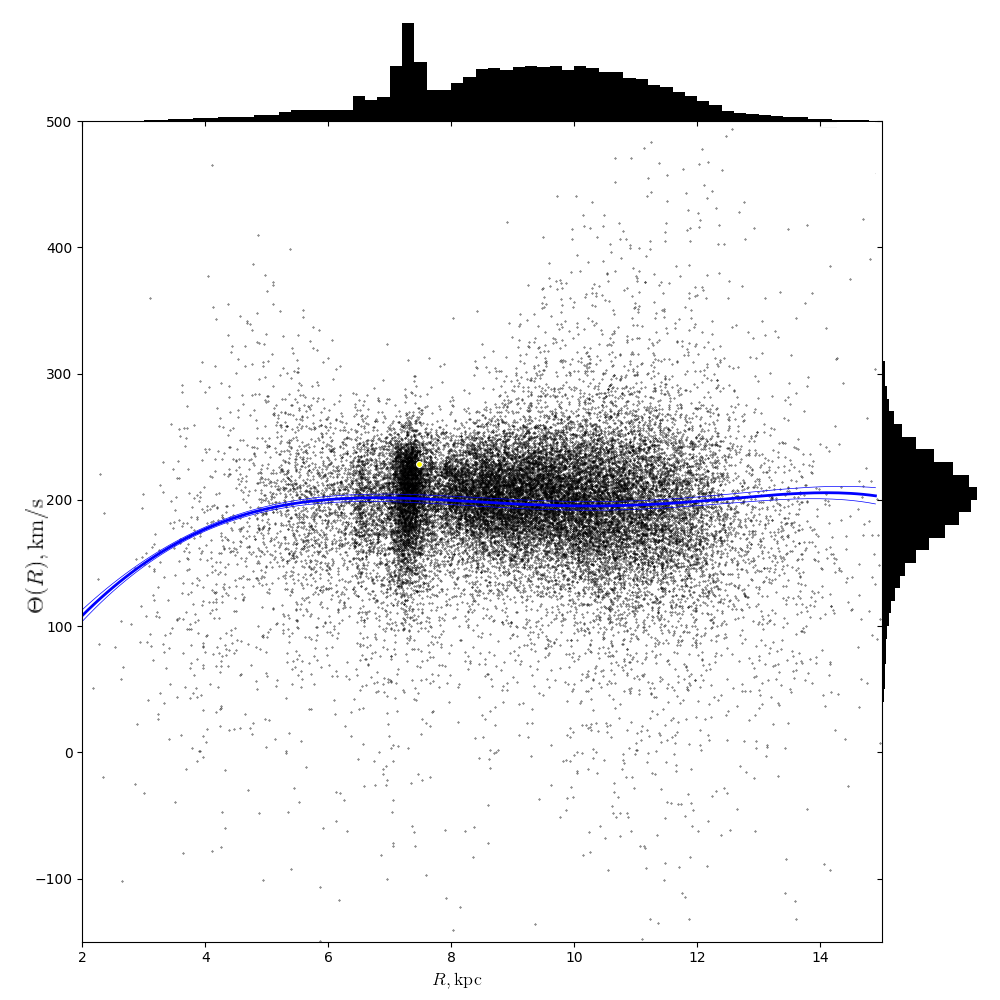
\includegraphics[width=1.0\textwidth]{../imgs/theta_obj.png}
\end{minipage}
\end{center}
\end{figure}
\end{frame}


\begin{frame}{Заключение}
        \Fontvi
\begin{enumerate}
        \item Выполнено обобщение на трехмерное поле скоростей метода пространственно-кинематического моделирования однородной плоской подсистемы объектов Галактики. Метод применен к данным каталога звезд красного сгущения (ЗКС) APOGEE-RC DR-14.
        \item Сравнение оценок параметра Оорта $A$, полученных из анализа по отдельности поля лучевых скоростей и поля собственных движений по долготе, свидетельствует в пользу заниженности в среднем шкалы расстояний для ЗКС. Однако поправочный коэффициент $K_A = 1.044 \pm 0.036$ незначимо отличается от единицы. Вместе с тем, оценки $R_0$, которые \textbf{впервые} удалось получить по долготным собственным движениям, превосходят оценки $R_0$ по лучевым скоростям, что поддерживает гипотезу о заниженности использованой шкалы расстояний. 
        \item Пространственно-кинематическое моделирование подсистемы ЗКС приводит к оценке расстояния от Солнца до центра Галактики $R_0$ в оригинальной шкале
                \begin{equation}
                        R_0 = 7.516^{+0.072}_{-0.090}|_{\mathrm{stat}} \pm 0.25 |_{\mathrm{calib}} , \nonumber
                \end{equation}
                c вероятной поправкой шкалы расстояний
                \begin{equation}
                        R_0 = 7.838^{+0.101}_{-0.088}|_{\mathrm{stat}} \pm 0.28 |_{\mathrm{calib}} . \nonumber
                \end{equation}
\item Большая протяженность области, представленой данными каталога APOGEE-RC DR-14, позволила исследовать кинематику Галактики на значительном промежутке расстояний, и построить статистически точную среднюю кривую вращения на отрезке ${\approx}12$ кпк в радиальном направлении. Построенная на интервале галактоцентрических расстояний $3\div15$ кпк по трехмерному полю скоростей кривая вращения \textit{плоская} на отрезке от 6 до 14 кпк, с незначительным спадом. Мелкомасштабной структуры кривой вращения \textit{не выявлено}.
\end{enumerate}
\end{frame}


%\begin{frame}{Ссылки}
% \begin{thebibliography}{10}
%\beamertemplatebookbibitems
%\bibitem{1} {\sc APOGEE-RC} {\em https://data.sdss.org/sas/dr13/apogee/vac/apogee-rc/cat/}
%\bibitem{2} {\sc Bovy and etc.} {\em http://adsabs.harvard.edu/abs/2014arXiv1405.1032B}
%\bibitem{3} {\sc Loktin A. V., Marsakov V. A. 2010} {Lectures on Stellar Astronomy, Rostov-na-Donu, pp. 282 (in Russian)}
%\bibitem{3} {\sc Gromov A.O., Nikiforov I.I. 2016} {STÄCKEL-TYPE DYNAMIC MODEL OF THE GALAXY BASED
%ON MASER KINEMATIC DATA}
%
%\end{thebibliography}
%\end{frame}

\begin{frame}{Маргинальные распределения}
%        \Fontvi
\begin{figure}[h!!]
\begin{center}
        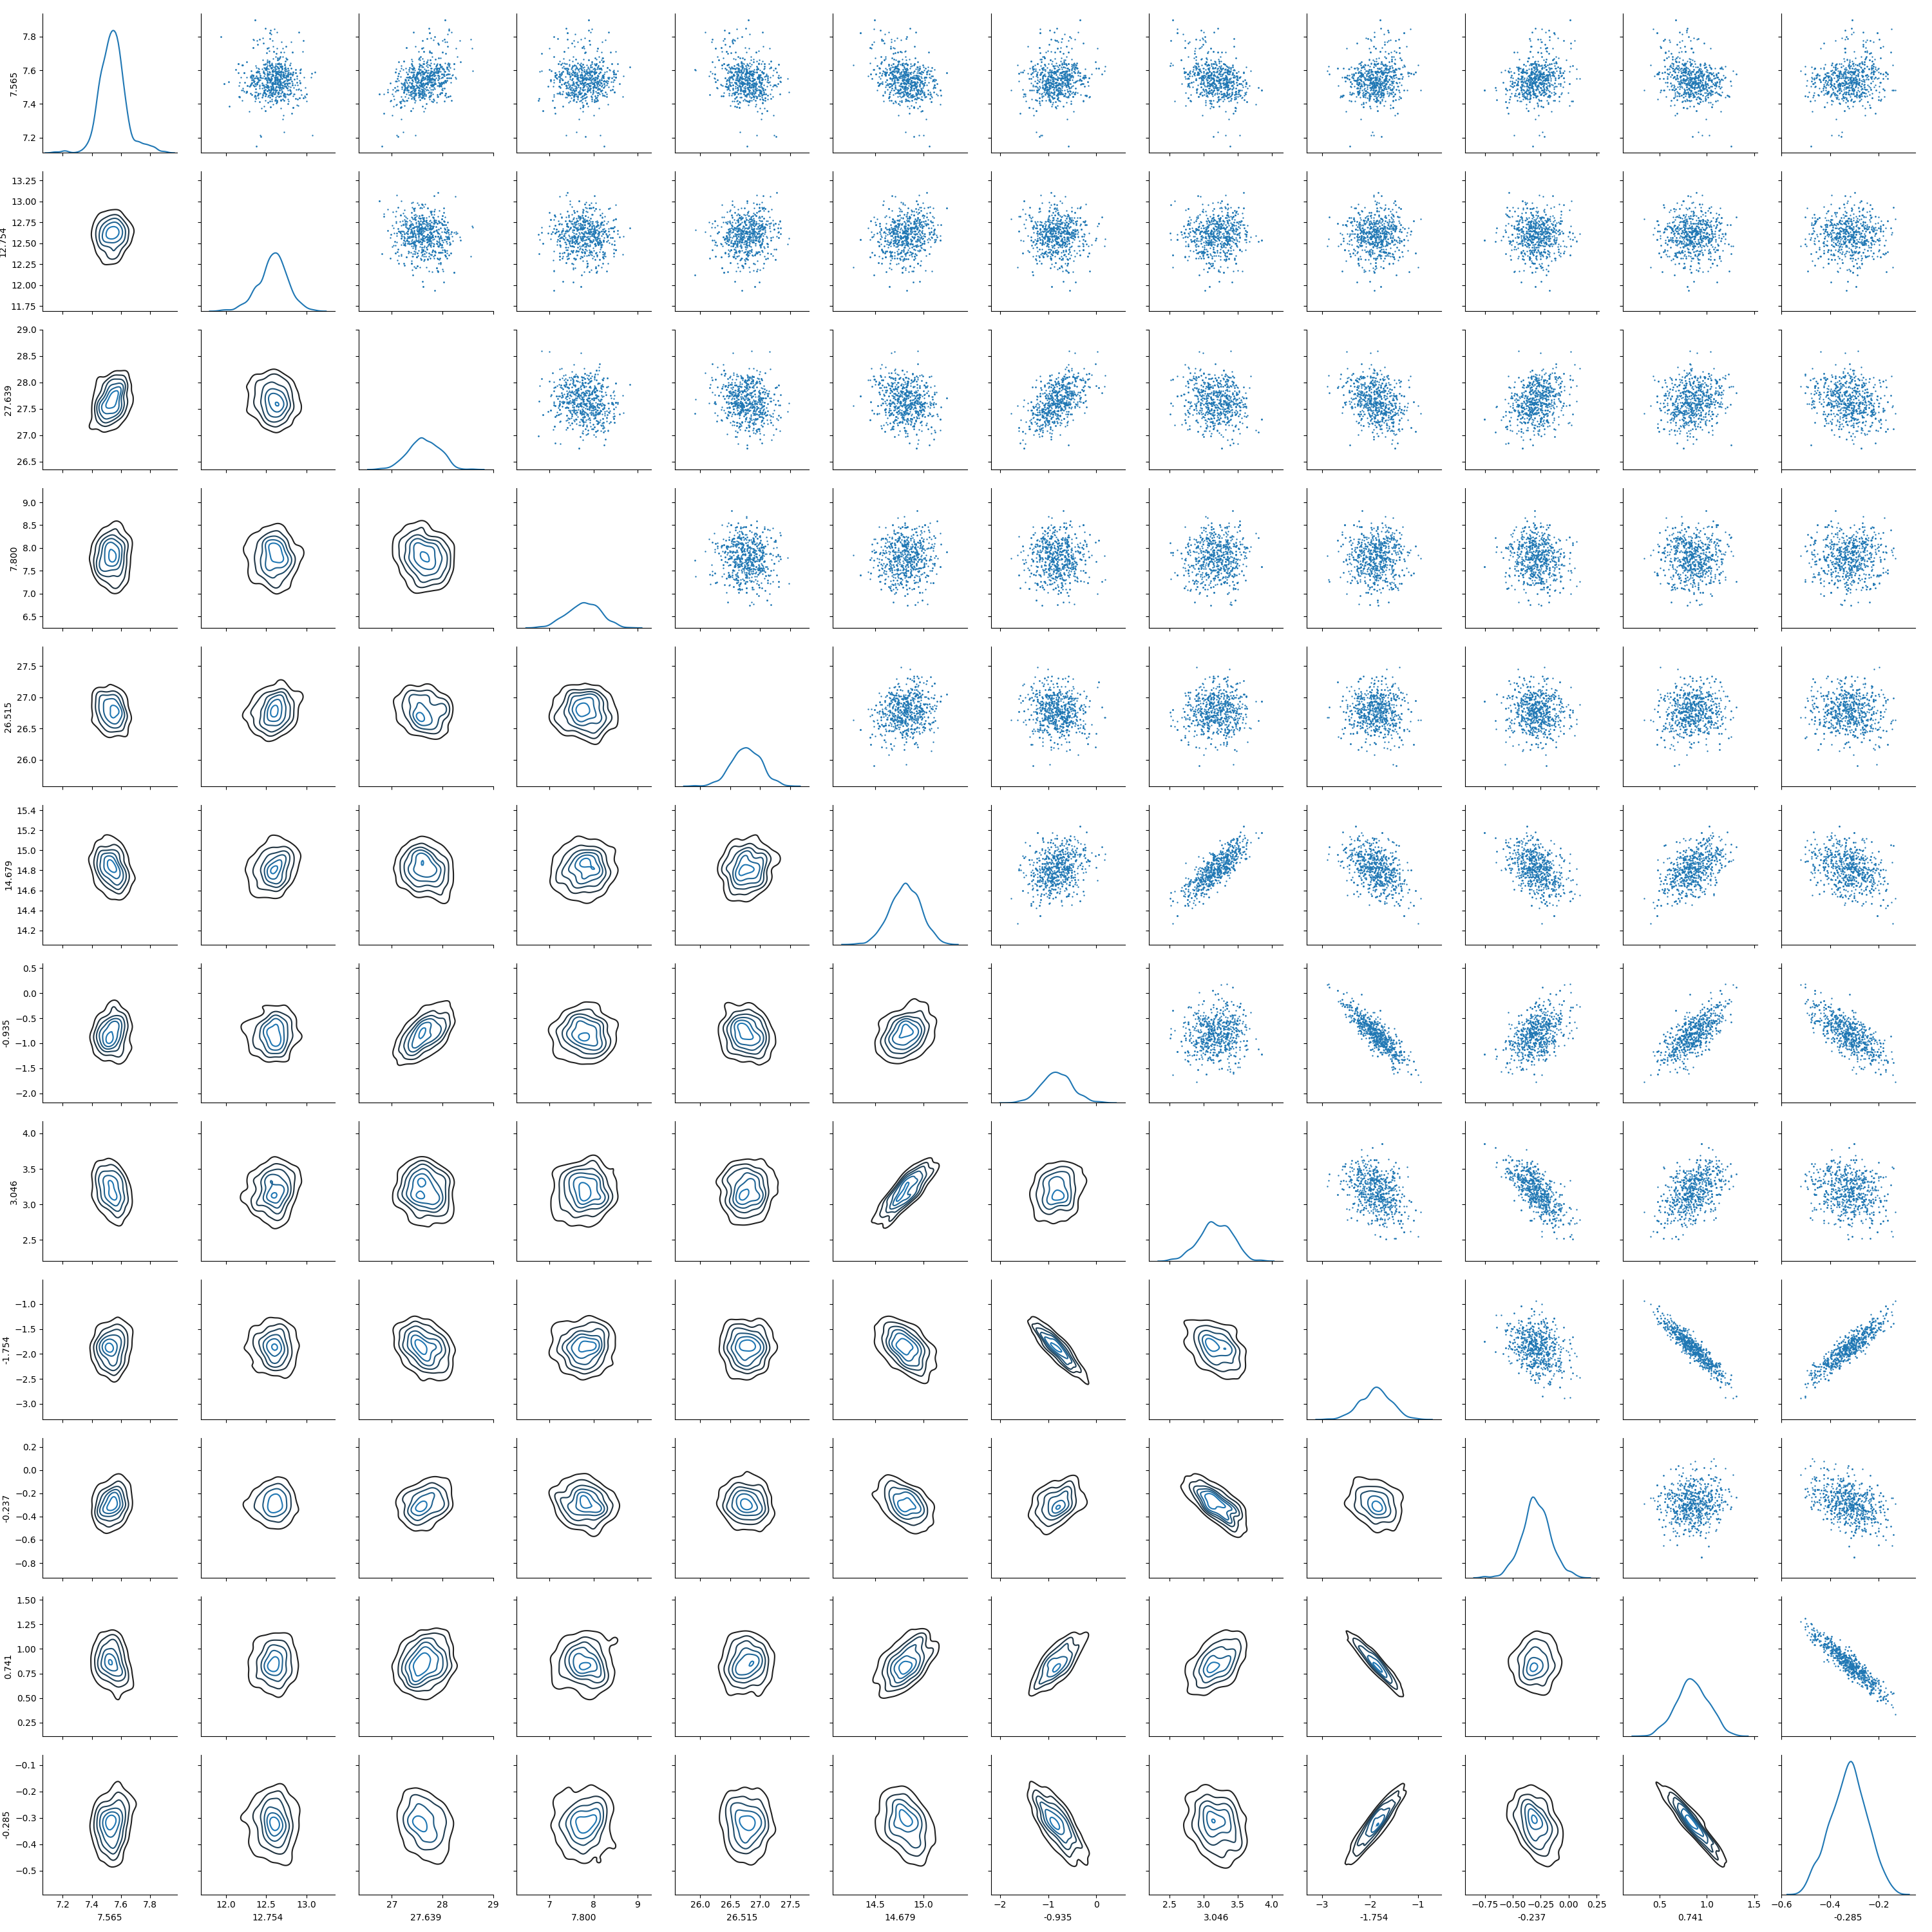
\includegraphics[width=0.7\textwidth]{../imgs/pairplot.png}
\end{center}
\end{figure}

\end{frame}


%\begin{frame}{APOGEE-RC}
%	\begin{figure}[h]
%\begin{minipage}[h]{0.8\linewidth}
%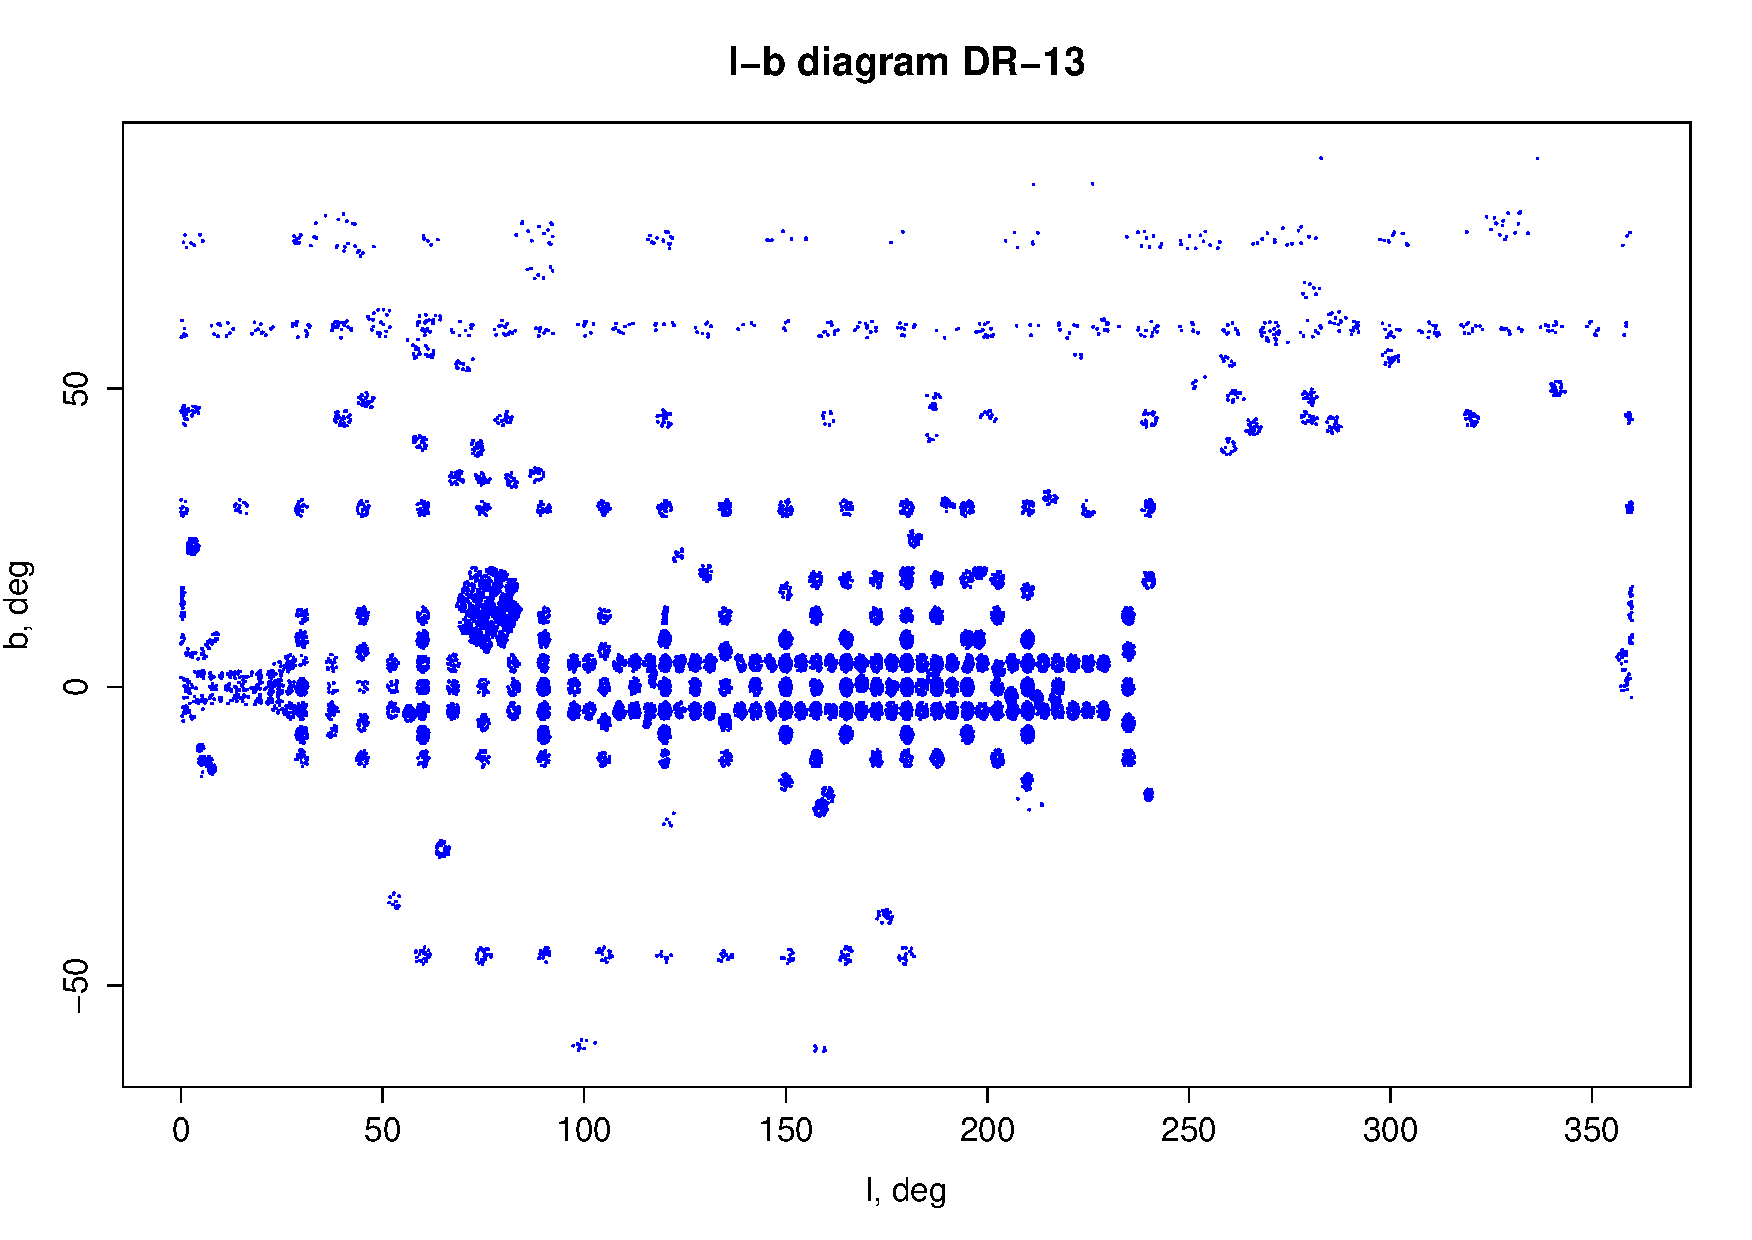
\includegraphics[width=1\linewidth]{pdf/lb_dr13.pdf}
%\end{minipage}
%\end{figure}
%\end{frame}

\end{document}
